% ===================================================================
%  Week 14 — Object Detection & Localization
%  Session 2 of 2: From sliding windows to single-shot detectors (YOLO), + mAP
%  Compile: pdflatex -interaction=nonstopmode slides-b.tex  (twice)
% ===================================================================
\documentclass[10pt,aspectratio=169]{beamer}
% ===================================================================
%  Shared Beamer preamble for "Practical Image Processing"
%  English slides. Compile with pdfLaTeX.
% ===================================================================

\usetheme{metropolis}
\usepackage[T1]{fontenc}
\usepackage[utf8]{inputenc}
\usepackage{lmodern}
\usepackage{listings}
\usepackage{tcolorbox}
\usepackage{fontawesome5}
\usepackage{booktabs}
\usepackage{amsmath,amssymb}
\usepackage{tikz}
\usepackage{pgfplots}
\pgfplotsset{compat=1.17}
\usetikzlibrary{arrows.meta,positioning,shapes.geometric,fit,backgrounds,matrix}
\tcbuselibrary{skins,breakable}

% ---- Palette --------------------------------------------------------
\definecolor{coursePrimary}{HTML}{1B4965}   % deep blue
\definecolor{courseAccent}{HTML}{E76F51}    % coral
\definecolor{courseGood}{HTML}{2A9D8F}      % teal
\definecolor{courseBad}{HTML}{C0392B}       % red
\definecolor{courseInfo}{HTML}{2980B9}      % blue
\definecolor{codeBg}{HTML}{F5F6FA}
\definecolor{codeKw}{HTML}{8E44AD}
\definecolor{codeStr}{HTML}{2A9D8F}
\definecolor{codeCom}{HTML}{7F8C8D}

\setbeamercolor{frametitle}{bg=coursePrimary}
\setbeamercolor{progress bar}{fg=courseAccent}
\setbeamercolor{alerted text}{fg=courseAccent}
\metroset{block=fill,sectionpage=progressbar,numbering=fraction}

% ---- Code listings (Python is built into listings) -----------------
\lstdefinestyle{course}{
  backgroundcolor=\color{codeBg},
  basicstyle=\ttfamily\scriptsize,
  keywordstyle=\color{codeKw}\bfseries,
  stringstyle=\color{codeStr},
  commentstyle=\color{codeCom}\itshape,
  numberstyle=\tiny\color{codeCom},
  numbers=left, numbersep=6pt,
  showstringspaces=false, breaklines=true, breakatwhitespace=true,
  tabsize=4, columns=fullflexible,
  frame=single, framesep=4pt, rulecolor=\color{gray!30},
  keepspaces=true, upquote=true, language=Python,
}
\lstset{style=course}
\lstdefinelanguage{bash}{
  keywords={cd,pip,python,venv,source,import}, sensitive=true,
  morecomment=[l]{\#}, morestring=[b]', morestring=[b]",
}

% ---- Reusable callout boxes ----------------------------------------
\newtcolorbox{goodbox}[1][Good practice]{colback=courseGood!8,colframe=courseGood,
  fonttitle=\bfseries,title={\faCheck~#1},boxrule=0.6pt,left=4pt,right=4pt,top=3pt,bottom=3pt}
\newtcolorbox{badbox}[1][Pitfall]{colback=courseBad!8,colframe=courseBad,
  fonttitle=\bfseries,title={\faTimes~#1},boxrule=0.6pt,left=4pt,right=4pt,top=3pt,bottom=3pt}
\newtcolorbox{infobox}[1][Note]{colback=courseInfo!8,colframe=courseInfo,
  fonttitle=\bfseries,title={\faInfoCircle~#1},boxrule=0.6pt,left=4pt,right=4pt,top=3pt,bottom=3pt}
\newtcolorbox{mathbox}[1][Math]{colback=coursePrimary!6,colframe=coursePrimary,
  fonttitle=\bfseries,title={\faCalculator~#1},boxrule=0.6pt,left=4pt,right=4pt,top=3pt,bottom=3pt}

\newcommand{\keyidea}[1]{\begin{alertblock}{Key idea}#1\end{alertblock}}
\newcommand{\term}[1]{\textbf{\color{coursePrimary}#1}}
\newcommand{\code}[1]{\lstinline[basicstyle=\ttfamily\small]|#1|}

% ---- A helper to draw a small pixel grid, cells shaded by value ----
% \pixelgrid{ {10,20,120,200,240}, {30,60,130,180,230}, ... }
\newcommand{\pixelgrid}[1]{%
  \begin{tikzpicture}[font=\scriptsize,scale=0.6]
    \foreach \row [count=\ry] in {#1} {
      \foreach \val [count=\cx] in \row {
        \draw[gray,fill=coursePrimary!8] (\cx,-\ry) rectangle ++(1,-1);
        \node at (\cx+0.5,-\ry-0.5) {\val};
      }
    }
  \end{tikzpicture}}


\title{Object Detection \& Localization}
\subtitle{Week 14 — Session 2: Single-shot detectors (YOLO) and measuring them (mAP)}
\author{Practical Image Processing}
\date{Lecture 14.2 \textbullet\ 60--70 min}

\begin{document}

\maketitle

\begin{frame}{Recap of Session 1}
  \begin{columns}[T]
    \begin{column}{0.58\textwidth}
      \begin{itemize}
        \item Detection = classify \emph{and} localize --- a variable number of boxes.
        \item A box is 4 numbers; localization is regression on them.
        \item \term{Sliding window} sweeps a classifier everywhere over an image pyramid --- correct but slow.
        \item \term{IoU} scores overlap; \term{NMS} collapses duplicate boxes into final detections.
      \end{itemize}
    \end{column}
    \begin{column}{0.42\textwidth}
      \begin{alertblock}{Today's job}
        Replace the brute-force sweep with \emph{one} CNN forward pass (YOLO), then learn to \emph{measure} a detector honestly with mAP --- and detect the DocScan digit strip.
      \end{alertblock}
    \end{column}
  \end{columns}
\end{frame}

\begin{frame}{Roadmap --- Session 2}\tableofcontents\end{frame}

% ==================================================================
\section{From proposals to single-shot}
% ==================================================================

\begin{frame}{First fix: propose, don't sweep}
  \begin{itemize}
    \item Sliding window tests \emph{every} location and scale --- most are empty background.
    \item \term{Region proposals} (e.g. \term{selective search}) suggest a few thousand ``objecty'' boxes first.
    \item Run the CNN only on those --- huge saving vs. hundreds of thousands of windows.
  \end{itemize}
  \begin{mathbox}[The two-stage family: R-CNN $\to$ Fast $\to$ Faster R-CNN]
    Stage 1: \emph{where might objects be?} \quad Stage 2: \emph{what is in each proposal + refine its box.}
  \end{mathbox}
  \keyidea{Two-stage detectors are accurate but still run a classifier once per proposal.}
\end{frame}

\begin{frame}{A detector timeline (intuition, not dates to memorize)}
  \begin{center}
  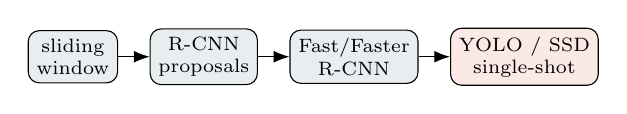
\begin{tikzpicture}[font=\scriptsize,node distance=4mm,
      s/.style={draw,rounded corners,fill=coursePrimary!10,minimum height=6mm,inner sep=3pt,align=center}]
    \node[s] (a) {sliding\\window};
    \node[s,right=of a] (b) {R-CNN\\proposals};
    \node[s,right=of b] (c) {Fast/Faster\\R-CNN};
    \node[s,right=of c,fill=courseAccent!15] (d) {YOLO / SSD\\single-shot};
    \draw[-{Latex[length=2mm]}] (a)--(b);
    \draw[-{Latex[length=2mm]}] (b)--(c);
    \draw[-{Latex[length=2mm]}] (c)--(d);
  \end{tikzpicture}
  \end{center}
  \begin{itemize}
    \item Each step removes redundant work: fewer windows, then shared features, then one pass.
    \item The \emph{ideas} stack --- IoU, NMS, and anchors carry all the way across this line.
  \end{itemize}
  \keyidea{The field's whole arc is ``do the same detection, but cheaper.''}
\end{frame}

\begin{frame}{Second fix: skip stages --- single-shot}
  \begin{itemize}
    \item \term{Single-shot} detectors (\term{YOLO}, \term{SSD}) do it all in \emph{one} forward pass.
    \item No separate proposal step: the CNN outputs boxes \emph{and} classes directly.
    \item Fast enough for video --- ``You Only Look Once.''
  \end{itemize}
  \begin{center}
  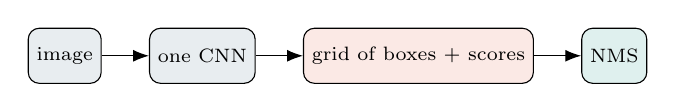
\begin{tikzpicture}[font=\scriptsize,node distance=6mm and 6mm,
      box/.style={draw,rounded corners,fill=coursePrimary!10,minimum height=7mm,inner sep=3pt}]
    \node[box] (img) {image};
    \node[box,right=of img] (cnn) {one CNN};
    \node[box,right=of cnn,fill=courseAccent!15] (out) {grid of boxes + scores};
    \node[box,right=of out,fill=courseGood!15] (nms) {NMS};
    \draw[-{Latex[length=2mm]}] (img)--(cnn);
    \draw[-{Latex[length=2mm]}] (cnn)--(out);
    \draw[-{Latex[length=2mm]}] (out)--(nms);
  \end{tikzpicture}
  \end{center}
  \keyidea{Trade a little accuracy for a lot of speed --- and NMS still cleans up at the end.}
\end{frame}

% ==================================================================
\section{How YOLO sees an image}
% ==================================================================

\begin{frame}{The grid idea}
  \begin{columns}[T]
    \begin{column}{0.5\textwidth}
      \begin{itemize}
        \item Divide the image into an $S\times S$ grid (here $3\times3$).
        \item The cell that contains an object's \emph{centre} is responsible for detecting it.
        \item Each cell predicts a few boxes relative to itself, plus class scores.
      \end{itemize}
    \end{column}
    \begin{column}{0.5\textwidth}
      \begin{center}
      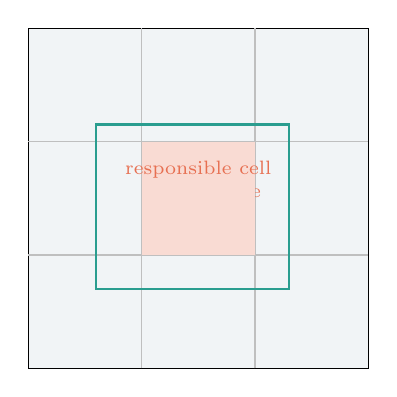
\begin{tikzpicture}[font=\scriptsize,scale=0.72]
        \draw[fill=coursePrimary!6] (0,0) rectangle (6,6);
        \foreach \i in {2,4} {\draw[gray!50] (\i,0)--(\i,6); \draw[gray!50] (0,\i)--(6,\i);}
        % object box + responsible cell
        \draw[thick,courseGood] (1.2,1.4) rectangle (4.6,4.3);
        \fill[courseAccent] (2.9,2.85) circle (3pt) node[above right,courseAccent]{centre};
        \fill[courseAccent!25] (2,2) rectangle (4,4);
        \node[courseAccent] at (3,3.5){responsible cell};
      \end{tikzpicture}
      \end{center}
    \end{column}
  \end{columns}
\end{frame}

\begin{frame}{What each cell predicts}
  For every cell, for each of its $B$ boxes:
  \begin{center}
  \begin{tabular}{@{}ll@{}}
    \toprule
    \textbf{Prediction} & \textbf{Meaning} \\
    \midrule
    $t_x,t_y$ & box centre, \emph{offset inside the cell} ($0$--$1$) \\
    $t_w,t_h$ & box width/height (relative to the image or an anchor) \\
    objectness $p_o$ & ``is there \emph{any} object here?'' confidence \\
    class scores $p_1..p_C$ & ``if there is, which class?'' \\
    \bottomrule
  \end{tabular}
  \end{center}
  \begin{mathbox}[Box confidence used for NMS]
    $\text{score}=p_o\times p_{\text{class}}$ \quad --- objectness times class probability
  \end{mathbox}
\end{frame}

\begin{frame}{The output tensor, counted}
  \begin{mathbox}[One grid, one tensor]
    output shape $=S\times S\times\big(B\cdot5 + C\big)$
  \end{mathbox}
  \begin{itemize}
    \item The $5$ = $(t_x,t_y,t_w,t_h,p_o)$ per box; $C$ = one class score set per cell.
    \item DocScan example: $S{=}7$, $B{=}2$ boxes, $C{=}2$ classes (document, digit-strip):
      \[ 7\times7\times(2\cdot5+2)=7\times7\times12 = 588 \text{ numbers.} \]
    \item One CNN forward pass produces \emph{all} of it at once --- no sweeping.
  \end{itemize}
  \keyidea{Detection becomes ``predict one fixed-size tensor,'' then decode + NMS it.}
\end{frame}

\begin{frame}{Anchor boxes: priors for shape}
  \begin{columns}[T]
    \begin{column}{0.55\textwidth}
      \begin{itemize}
        \item Objects have typical shapes: a digit strip is \emph{wide}, a dial is \emph{square}.
        \item \term{Anchors} are a few preset box shapes per cell; the net predicts a small \emph{correction} to an anchor, not a box from scratch.
        \item Easier to learn a nudge than an absolute size --- and different anchors specialize in different shapes.
      \end{itemize}
    \end{column}
    \begin{column}{0.45\textwidth}
      \begin{center}
      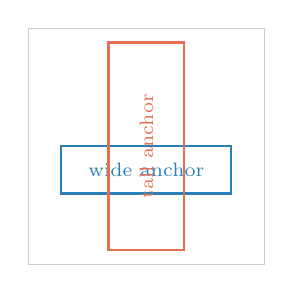
\begin{tikzpicture}[font=\scriptsize,scale=0.6]
        \draw[gray!40] (0,0) rectangle (5,5);
        \draw[courseInfo,thick] (0.7,1.5) rectangle (4.3,2.5);
        \node[courseInfo] at (2.5,2){wide anchor};
        \draw[courseAccent,thick] (1.7,0.3) rectangle (3.3,4.7);
        \node[courseAccent,rotate=90] at (2.5,2.5){tall anchor};
      \end{tikzpicture}
      \end{center}
    \end{column}
  \end{columns}
  \keyidea{An anchor is an educated guess about a box's shape; the net only refines it.}
\end{frame}

\begin{frame}{Training a single-shot detector (intuition)}
  \begin{itemize}
    \item Assign each ground-truth object to the cell/anchor with best \term{IoU}.
    \item Loss has three parts, summed:
    \begin{itemize}
      \item \emph{box} loss (regression) for the responsible box;
      \item \emph{objectness} loss ($p_o\to1$ where an object is, $\to0$ elsewhere);
      \item \emph{class} loss (cross-entropy) for the responsible cell.
    \end{itemize}
    \item Most cells are background $\Rightarrow$ weight objectness carefully or the net predicts ``nothing.''
  \end{itemize}
  \begin{mathbox}
    $L = \lambda_{\text{box}}L_{\text{box}} + L_{\text{obj}} + L_{\text{cls}}$
  \end{mathbox}
\end{frame}

\begin{frame}{At inference: decode, then NMS}
  \begin{enumerate}
    \item Forward pass $\rightarrow$ the $S\times S\times(B\cdot5+C)$ tensor.
    \item For each box: $\text{score}=p_o\times p_{\text{class}}$; drop scores below a threshold.
    \item Convert cell-relative $(t_x,t_y,t_w,t_h)$ to absolute pixel boxes.
    \item Run \term{NMS} per class --- exactly Session 1's algorithm.
  \end{enumerate}
  \begin{goodbox}
    The detector proposes; NMS disposes. Session 1's two tools are still doing the final cleanup.
  \end{goodbox}
\end{frame}

\begin{frame}{Two different knobs (do not confuse them)}
  \begin{columns}[T]
    \begin{column}{0.5\textwidth}
      \begin{infobox}[Confidence threshold]
        Applied \emph{before} NMS to each box's $\text{score}=p_o\times p_{\text{class}}$. Raise it $\rightarrow$ fewer, more certain boxes (fewer false positives, more misses).
      \end{infobox}
    \end{column}
    \begin{column}{0.5\textwidth}
      \begin{infobox}[NMS IoU threshold $\tau$]
        Applied \emph{during} NMS between surviving boxes. Raise it $\rightarrow$ more overlaps allowed to coexist (more duplicates in crowds).
      \end{infobox}
    \end{column}
  \end{columns}
  \vspace{3pt}
  \begin{badbox}
    ``Too many boxes'' has two cures --- raise the \emph{confidence} threshold, or lower the \emph{NMS} threshold. They fix different problems; know which one you are turning.
  \end{badbox}
\end{frame}

% ==================================================================
\section{Measuring a detector: mAP}
% ==================================================================

\begin{frame}{A detection is right only if the box is right}
  \begin{itemize}
    \item A prediction counts as a \term{true positive} if its IoU with a ground-truth box $\ge$ a threshold (usually $0.5$) \emph{and} the class matches.
    \item Otherwise it is a \term{false positive}; a missed ground-truth is a \term{false negative}.
    \item Only \emph{one} prediction may claim each ground-truth box --- extra ones are false positives.
  \end{itemize}
  \begin{mathbox}[Precision \& recall]
    $\text{precision}=\dfrac{TP}{TP+FP}, \qquad \text{recall}=\dfrac{TP}{TP+FN}$
  \end{mathbox}
\end{frame}

\begin{frame}{Precision \& recall, worked}
  5 predictions ranked by score; 3 ground-truth objects; IoU$\ge0.5$ = a hit.
  \begin{center}
  \begin{tabular}{@{}clccc@{}}
    \toprule
    \textbf{Rank} & \textbf{Result} & \textbf{cum TP} & \textbf{Precision} & \textbf{Recall} \\
    \midrule
    1 & TP & 1 & $1/1=1.00$ & $1/3=0.33$ \\
    2 & TP & 2 & $2/2=1.00$ & $2/3=0.67$ \\
    3 & FP & 2 & $2/3=0.67$ & $0.67$ \\
    4 & TP & 3 & $3/4=0.75$ & $3/3=1.00$ \\
    5 & FP & 3 & $3/5=0.60$ & $1.00$ \\
    \bottomrule
  \end{tabular}
  \end{center}
  As we accept lower-scored boxes, recall rises but precision tends to fall --- the classic trade-off.
\end{frame}

\begin{frame}{The precision--recall curve and AP}
  \begin{columns}[T]
    \begin{column}{0.55\textwidth}
      \begin{center}
      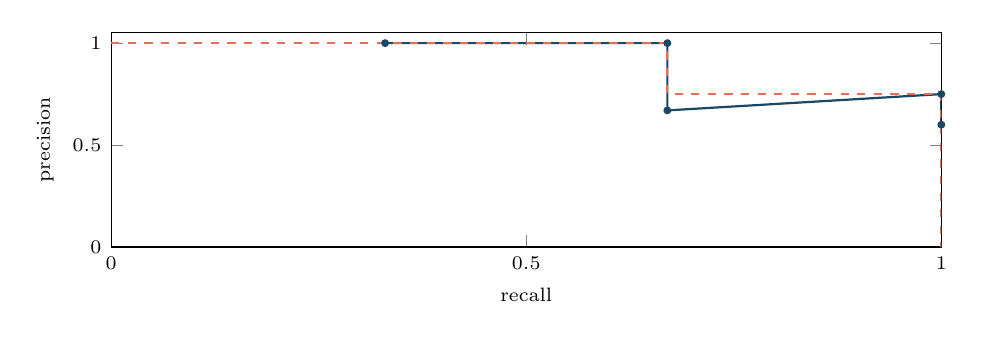
\begin{tikzpicture}
        \begin{axis}[width=\linewidth,height=4.3cm,xlabel={recall},ylabel={precision},
            tick label style={font=\scriptsize},label style={font=\scriptsize},
            xmin=0,xmax=1,ymin=0,ymax=1.05,ytick={0,0.5,1},xtick={0,0.5,1}]
          \addplot[coursePrimary,thick,mark=*,mark size=1pt] coordinates
            {(0.33,1.0)(0.67,1.0)(0.67,0.67)(1.0,0.75)(1.0,0.6)};
          \addplot[courseAccent,thick,dashed] coordinates
            {(0,1.0)(0.67,1.0)(0.67,0.75)(1.0,0.75)(1.0,0)};
        \end{axis}
      \end{tikzpicture}
      \end{center}
    \end{column}
    \begin{column}{0.45\textwidth}
      \begin{itemize}
        \item \term{Average Precision (AP)} = area under the (interpolated) PR curve.
        \item Coral: the ``max precision to the right'' interpolation used in practice.
        \item \term{mAP} = mean AP across all classes.
      \end{itemize}
    \end{column}
  \end{columns}
\end{frame}

\begin{frame}{mAP: the one number people quote}
  \begin{itemize}
    \item Compute AP \emph{per class}, then average $\rightarrow$ \term{mAP} (mean Average Precision).
    \item \code{mAP@0.5}: hits need IoU $\ge0.5$. \code{mAP@[.5:.95]}: average over many IoU thresholds (stricter, COCO-style).
    \item Higher mAP = better boxes \emph{and} better labels, in one score.
  \end{itemize}
  \begin{badbox}
    A high \emph{classification} accuracy says nothing about box quality. Detection must be judged with IoU-aware metrics like mAP --- never plain accuracy.
  \end{badbox}
\end{frame}

\begin{frame}{The precision--recall trade-off, in one picture}
  \begin{center}
  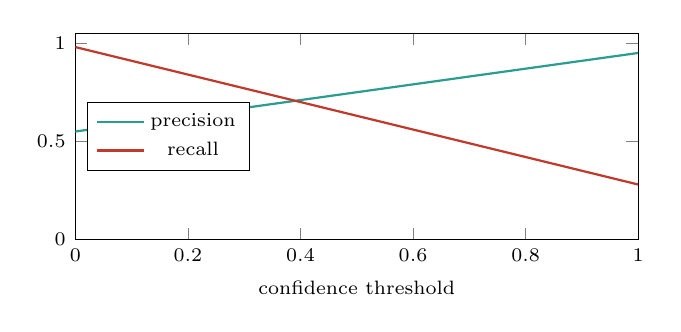
\begin{tikzpicture}
    \begin{axis}[width=0.72\linewidth,height=4.2cm,xlabel={confidence threshold},
        legend style={font=\scriptsize,at={(0.02,0.5)},anchor=west},
        tick label style={font=\scriptsize},label style={font=\scriptsize},
        ymin=0,ymax=1.05,xmin=0,xmax=1]
      \addplot[courseGood,thick,domain=0:1,samples=40] {0.55+0.4*x};
      \addplot[courseBad,thick,domain=0:1,samples=40] {0.98-0.7*x};
      \legend{precision,recall}
    \end{axis}
  \end{tikzpicture}
  \end{center}
  \begin{itemize}
    \item Raise the confidence threshold: precision climbs (fewer false positives), recall falls (more misses).
    \item mAP integrates over this whole sweep, so it does not hinge on one hand-picked threshold.
  \end{itemize}
\end{frame}

% ==================================================================
\section{Code: IoU and NMS from scratch}
% ==================================================================

\begin{frame}[fragile]{IoU in NumPy}
\begin{lstlisting}[language=Python]
def iou(a, b):                       # boxes as (x1, y1, x2, y2)
    ix1, iy1 = max(a[0], b[0]), max(a[1], b[1])
    ix2, iy2 = min(a[2], b[2]), min(a[3], b[3])
    iw, ih = max(0, ix2 - ix1), max(0, iy2 - iy1)   # clamp at 0
    inter = iw * ih
    area_a = (a[2]-a[0]) * (a[3]-a[1])
    area_b = (b[2]-b[0]) * (b[3]-b[1])
    return inter / (area_a + area_b - inter + 1e-9)
\end{lstlisting}
  \begin{itemize}
    \item The \code{max(0, ...)} clamp is the whole trick --- non-overlapping boxes give $0$.
    \item \code{+ 1e-9} avoids a divide-by-zero on degenerate (zero-area) boxes.
    \item This matches the by-hand result: $\text{iou}((1,1,5,4),(3,2,7,6))=0.167$.
  \end{itemize}
\end{frame}

\begin{frame}[fragile]{NMS in NumPy}
\begin{lstlisting}[language=Python]
def nms(boxes, scores, tau=0.5):
    order = sorted(range(len(scores)),           # high score first
                   key=lambda i: scores[i], reverse=True)
    keep = []
    while order:
        i = order.pop(0)                         # take the best
        keep.append(i)
        order = [j for j in order                # drop overlaps
                 if iou(boxes[i], boxes[j]) < tau]
    return keep
\end{lstlisting}
  \begin{itemize}
    \item Greedy: keep the top box, remove everything that overlaps it past $\tau$, repeat.
    \item Runs \emph{per class} --- never suppress a dial with a meter.
    \item Returns the indices of the surviving boxes --- the final detections.
  \end{itemize}
\end{frame}

\begin{frame}[fragile]{Localizing the digit strip (the DocScan tie-in)}
\begin{lstlisting}[language=Python]
# score every sliding window, then clean up with NMS
boxes, scores = [], []
for (x, y, w, h) in slide(img, win=(120, 40), stride=8):
    s = strip_score(img[y:y+h, x:x+w])   # "looks like a digit strip?"
    if s > 0.6:
        boxes.append((x, y, x+w, y+h)); scores.append(s)
keep = nms(boxes, scores, tau=0.4)       # collapse the cluster
strip = boxes[keep[0]]                    # feed this crop to Week 13's reader
\end{lstlisting}
  \begin{itemize}
    \item Same pipeline, tiny scale: sweep $\rightarrow$ score $\rightarrow$ NMS $\rightarrow$ one clean box.
    \item That one box is exactly the crop Week 13's digit CNN expects.
  \end{itemize}
\end{frame}

% ==================================================================
\section{In-class exercise}
% ==================================================================

\begin{frame}{\faPen~In-class exercise (10 min)}
  \begin{infobox}[Reason about detectors and their scores]
  \end{infobox}
  \begin{enumerate}
    \item A YOLO grid is $7\times7$ with $B{=}3$ boxes and $C{=}5$ classes. What is the output tensor size?
    \item Predictions ranked TP, FP, TP with 2 ground-truth objects. Give precision \& recall after each.
    \item Why must a detector be scored with mAP rather than plain classification accuracy?
    \item Your detector reports one meter as three boxes. Which knob do you reach for, and how?
  \end{enumerate}
\end{frame}

\begin{frame}{\faPen~Debrief}
  \begin{itemize}
    \item (1) $7\times7\times(3\cdot5+5)=7\times7\times20=980$ numbers.
    \item (2) TP: $P{=}1.00,R{=}0.5$; FP: $P{=}0.5,R{=}0.5$; TP: $P{=}0.67,R{=}1.0$.
    \item (3) Accuracy ignores \emph{where} the box is; mAP rewards correct class \emph{and} IoU-tight boxes, and balances precision vs recall over all thresholds.
    \item (4) \term{NMS}: the IoU threshold $\tau$ is too high --- lower it so the duplicate boxes get suppressed.
  \end{itemize}
  \keyidea{You can now size a detector's output, read its PR numbers, and debug its boxes.}
\end{frame}

% ==================================================================
\section{Wrap-up}
% ==================================================================

\begin{frame}{Two-stage vs single-shot --- an honest comparison}
  \begin{center}
  \begin{tabular}{@{}lll@{}}
    \toprule
    & \textbf{Two-stage (Faster R-CNN)} & \textbf{Single-shot (YOLO/SSD)} \\
    \midrule
    Speed    & slower & real-time \\
    Accuracy & typically higher & very close, improving \\
    Small objects & handles better & historically weaker \\
    Simplicity & pipeline of parts & one network \\
    \bottomrule
  \end{tabular}
  \end{center}
  \keyidea{Need real-time on a phone (DocScan)? Single-shot. Need every tiny object at any cost? Two-stage.}
\end{frame}

\begin{frame}{Pitfalls when building detectors}
  \begin{badbox}[Watch out]
    \begin{itemize}
      \item Judging a detector by accuracy instead of mAP --- boxes can be badly placed yet ``accurate.''
      \item Running NMS across classes, or forgetting it entirely (duplicate boxes everywhere).
      \item Ignoring the background/foreground imbalance --- the net learns to predict ``nothing.''
      \item Anchor shapes mismatched to your objects --- give a wide digit strip a wide anchor.
    \end{itemize}
  \end{badbox}
\end{frame}

\begin{frame}{What you should now be able to do}
  \begin{itemize}
    \item Explain the path from sliding windows $\rightarrow$ region proposals $\rightarrow$ single-shot detectors.
    \item Describe YOLO's grid, anchors, objectness, and its $S\times S\times(B\cdot5+C)$ output tensor.
    \item Decode + NMS a detector's output into final boxes.
    \item Score a detector with precision, recall, AP, and mAP --- and read a PR curve.
  \end{itemize}
\end{frame}

\begin{frame}{This week's deliverable}
  \begin{alertblock}{Due before the capstone finale (see \code{project/})}
    \begin{enumerate}
      \item Implement \code{iou} and \code{nms}; verify IoU on the by-hand boxes ($=0.167$) and disjoint boxes ($=0$).
      \item Run the sliding-window demo: localize the digit strip in a synthetic meter image, then NMS.
      \item Feed the localized crop to a digit reader (reuse Week 13) --- report the read value.
      \item Compute precision/recall for a small set of detections vs. ground truth; sketch the PR curve.
      \item Reflect: how does ``find the strip, then read it'' complete the DocScan pipeline?
    \end{enumerate}
  \end{alertblock}
\end{frame}

\begin{frame}[standout]
  Find it, then read it.\\[4pt]
  \normalsize One CNN sweep, decoded into boxes, cleaned by NMS, judged by mAP --- detection is Week 13 aimed at ``where.''
\end{frame}

\end{document}
